%%%%%%%%%%%%%%%%%%%%%%%%%%%%%%%%%%%%%%%%%%%%%%%%%%%%%%%%%%%%%%%%%%%%%%%%%%%%%%
%% Prunus METHODS AND PROTOCOLS - Pedro - 19 July 2006
%%%%%%%%%%%%%%%%%%%%%%%%%%%%%%%%%%%%%%%%%%%%%%%%%%%%%%%%%%%%%%%%%%%%%%%%%%%%%%
%%%%%%%%%%%%%%%%%%%%%%%%%%%%%%%%%%%%%%%%%%%%%%%%%%%%%%%%%%%%%%%%%%%%%% Headers
\documentclass[a4paper,12pt]{article}
\usepackage{amsmath,amssymb}
%\usepackage[utf8]{inputenc}
%\usepackage[applemac]{inputenc}
\usepackage{geometry}
\usepackage{lscape}
\usepackage{setspace}
\usepackage{framed}
\usepackage{verbatim}
\usepackage{graphicx}
\usepackage{epstopdf}
\usepackage{booktabs}
\usepackage{natbib}
\usepackage{longtable}
\usepackage{rotating}                                                                                    
\newcommand{\tab}{\hspace{5mm}}
\usepackage{tabularx} 
\usepackage[margin=10pt,font=small,labelfont=bf]{caption}
\usepackage[left,pagewise]{lineno}
\usepackage{caption}
\DeclareGraphicsRule{.tif}{png}{.png}{`convert #1 `basename #1 .tif`.png}
\usepackage{fancyhdr} % This should be set AFTER setting up the page geometry
\pagestyle{fancy}     % options: empty , plain , fancy
\renewcommand{\headrulewidth}{0pt} % customise the layout...
\lhead{{\tiny Jordano and Godoy - Prunus mahaleb study protocols}}\chead{}\rhead{}
\lfoot{}\cfoot{\thepage}\rfoot{}

%%%%%%%%%%%%%%%%%%%%%%%%%%%%%%%%%%%%%%%%%%%%%%%%%%%%%%%%%%%%%%%%%%% Title page
\begin{document}

\title{General methods for seed dispersal analysis and lab protocols 
for DNA extraction and genotyping of SSR microsatellites for 
\textit{Prunus mahaleb} (Rosaceae)}

\author{Pedro Jordano \& Jos\'e A. Godoy}

%%%\date{Sevilla, \today}
\maketitle


\begin{center}
{\small with the collaboration of: \textbf{Juan Miguel Arroyo}}{\small , \textbf{Cristina Garc\'{\i}a}}{\small , and additional help with field work from \textbf{Juan Luis Garc\'{\i}a-Casta\~{n}o}}{\small , \textbf{Jes\'{u}s G.P. Rodr\'{\i}guez}}{\small , and \textbf{Manuel Carri\'{o}n}}


\end{center}
\tab Contact address:
\begin{center}
Integrative Ecology Group, Estaci\'{o}n Biol\'{o}gica de Do\~{n}ana, 
CSIC, Pabell\'{o}n del Per\'{u}, Avda. M. Luisa S/N, E--41013 Sevilla, 
Spain

E-mail: jordano@ebd.csic.es, godoy@ebd.csic.es

\vspace{0.5cm}
$\texttt{\underline {http://ebd10.ebd.csic.es}} $\\
$\texttt{\underline {http://ieg.ebd.csic.es}}$\\
$\texttt{\underline {http://www.ebd.csic.es/lem}}$

\vspace{1cm}
\textbf{\textit{A separate document includes a detailed, step by step, 
description of the lab protocols.}}

\end{center}

\begin{center}
\textbf{{\small Acknowledgements}}
\end{center}

{\footnotesize Over the years, our work has been supported by grants PB96-0857, 1FD97-0743-C03-01, BOS2000-1366-C02-01, and REN2003-00273 from the Comisi\'{o}n Interministerial de Ciencia y Tec-nolog\'{\i}a, Ministerio de Educaci\'{o}n y Ciencia and the European Commission, and also by funds from the Consejer\'{\i}a de Educaci\'{o}n y Ciencia, Junta de Andaluc\'{\i}a (RNM305).}

\begin{center}
Version 1.5. Sevilla, July 2006.
\end{center}

%%%%%%%%%%%%%%%%%%%%%%%%%%%%%%%%%%%%%%%%%%%%%%%%%%%%%%%%%%%%%%%%%%%% MAIN TEXT
\section{Introduction}

This is a summary of our protocols for the genetic evaluation of seed dispersal in \textit{Prunus mahaleb} (Rosaceae). They combine seed sampling in the field by means of seed traps- that passively capture seeds dispersed (regurgitated or defecated) by frugivores- and genetic analysis of adult trees and seed endocarps. This enables us to identify uniquely the source tree for a dispersed seed. This method has been previously described in the companion papers (Godoy \& Jordano 2001, Jordano and Godoy 2002). Other applications of this approach can be found in the recent work by Ziegenhagen \textit{et al}. (2003), Grivet \textit{et al}. (2005) and Jones \textit{et al}. (2005).

\section{Study species}

The study species is \textit{Prunus mahaleb} (L.), a rosaceous tree that in SE Spanish populations is gynodioecious, with individuals producing hermaphrodite flowers and others with androsterile flowers, which behave as functional females. In the southern Iberian Peninsula this species flowers between mid-May and mid-June at high elevations (over 1300 m) and insects, mainly bees (Hymenoptera: Andrenidae, Apidae) and flies (Diptera: Calliphoridae, Syrphidae) act as pollen vectors. \textit{P. mahaleb} produces fleshy fruits (drupaceous) (Fig. 1) with 1 seed per fruit. In late July fleshy fruits are produced and consumed by frugivorous animals that disperse the seeds until late August or early September.

%------------------------------------------------------------------- Figure 1
\begin{figure}[htbp]
\centerline{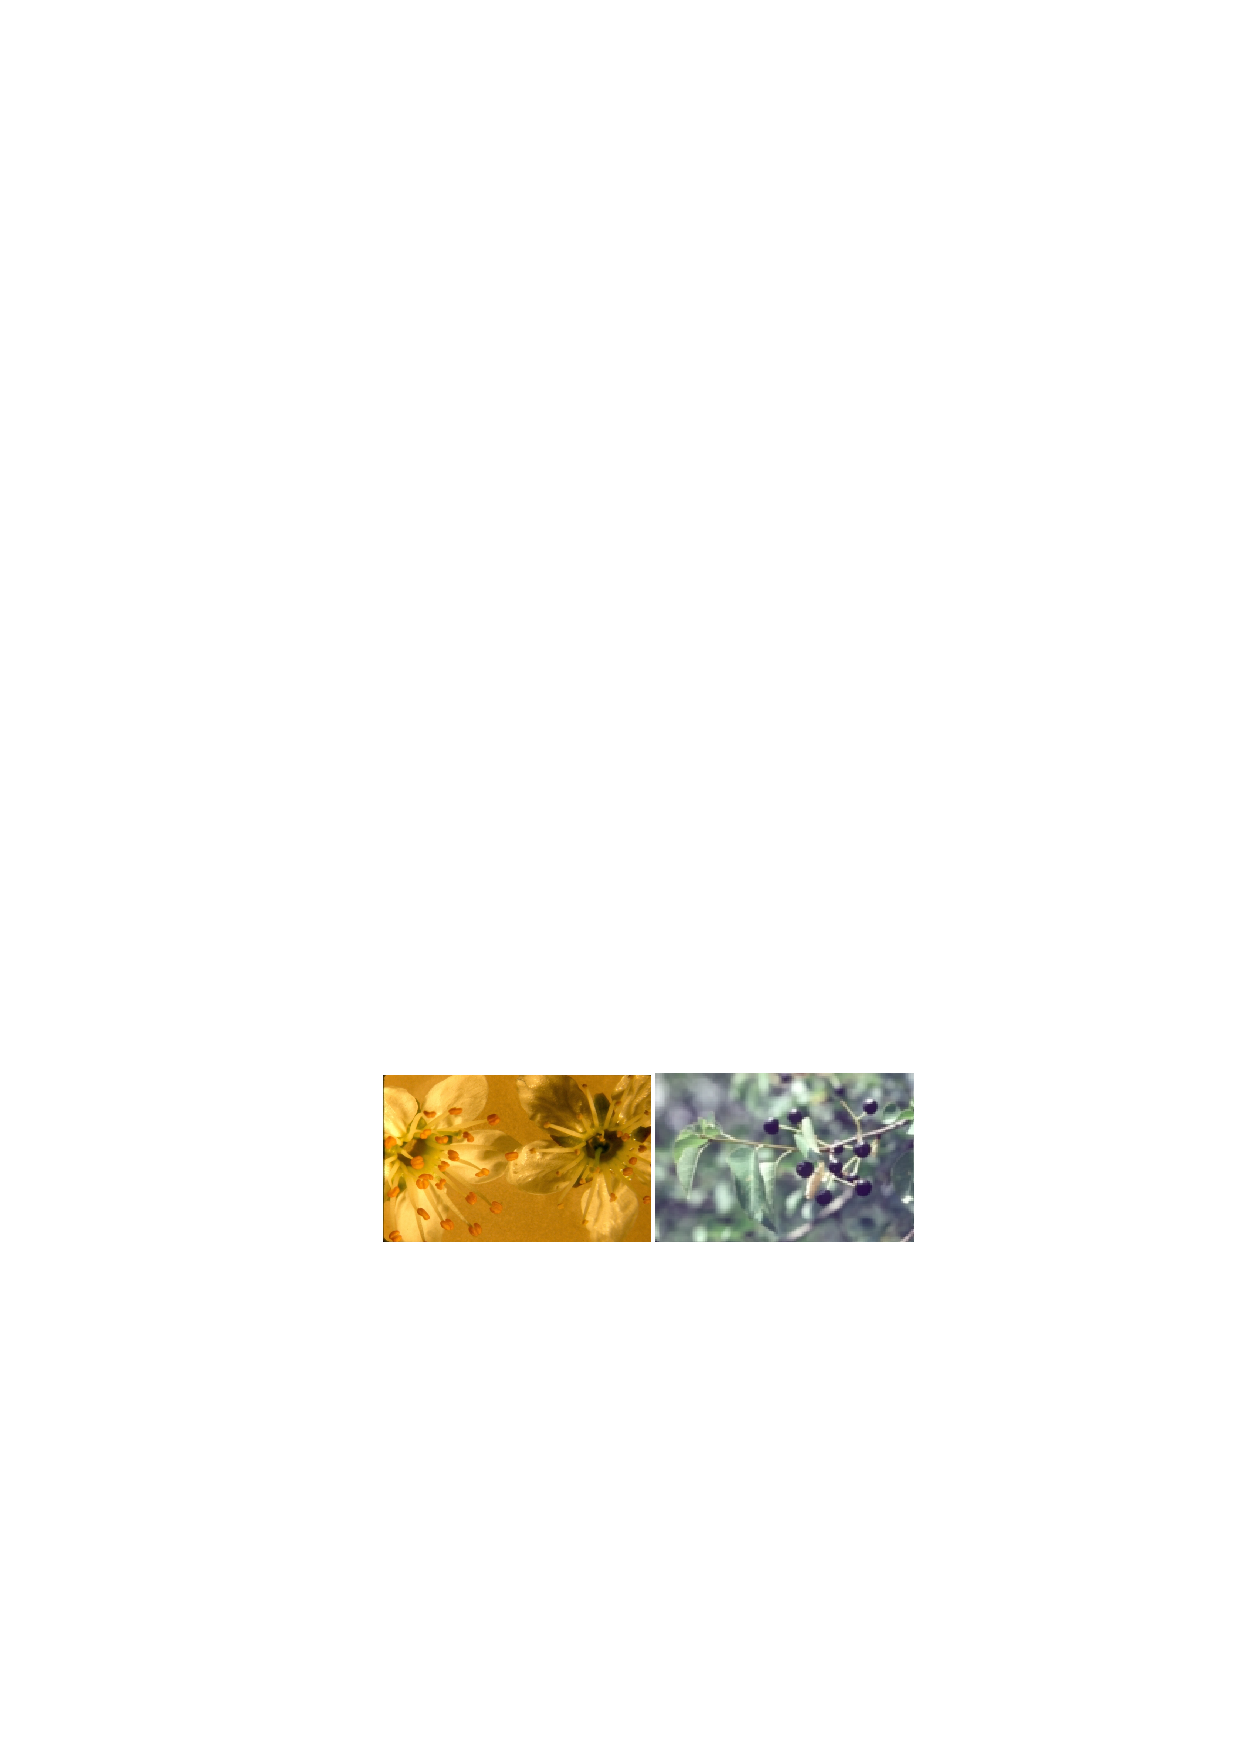
\includegraphics[height=3cm]{fig1.pdf}}
%
\caption{Flowers and ripe fruits of \textit{P. mahaleb}. Flowers show the typical hermaphrodite tree flower (left) and the androsterile flower (right) of a female tree, with anthers unfunctional and shrunken.}\end{figure}
%------------------------------------------------------------------- Figure 1


\section{Description of the main study population}

\tab Our 9 local \textit{Prunus mahaleb} populations are located in Parque Natural de las Sierras de Cazorla, Segura y Las Villas (Ja\'{e}n province, SE Spain). In this area \textit{P. mahaleb} naturally occurs as isolated small (10 trees) to medium-size (150 trees) distinct populations. A few populations might reach ca. 5000 trees. These populations are naturally isolated from each other and occupy an approximate extension of 150 $km^{2}$. The main study population was located in Nava de las Correhuelas (NCH), at 1615 m elevation. Detailed descriptions of the area and general methods can be found in Jordano (1994, 1995) and Jordano \& Schupp (2000). The site is dominated by grasslands with scattered patches of deciduous vegetation, gravely soil or rock outcrops covered by shrubs or small isolated trees (Fig. 2). The rocky slopes are dominated by open pine forest (\textit{Pinus nigra} subsp. \textit{salzmannii}) and juniper (\textit{Juniperus communis}).

%------------------------------------------------------------------- Figure 2
\begin{figure}[htbp]
\centerline{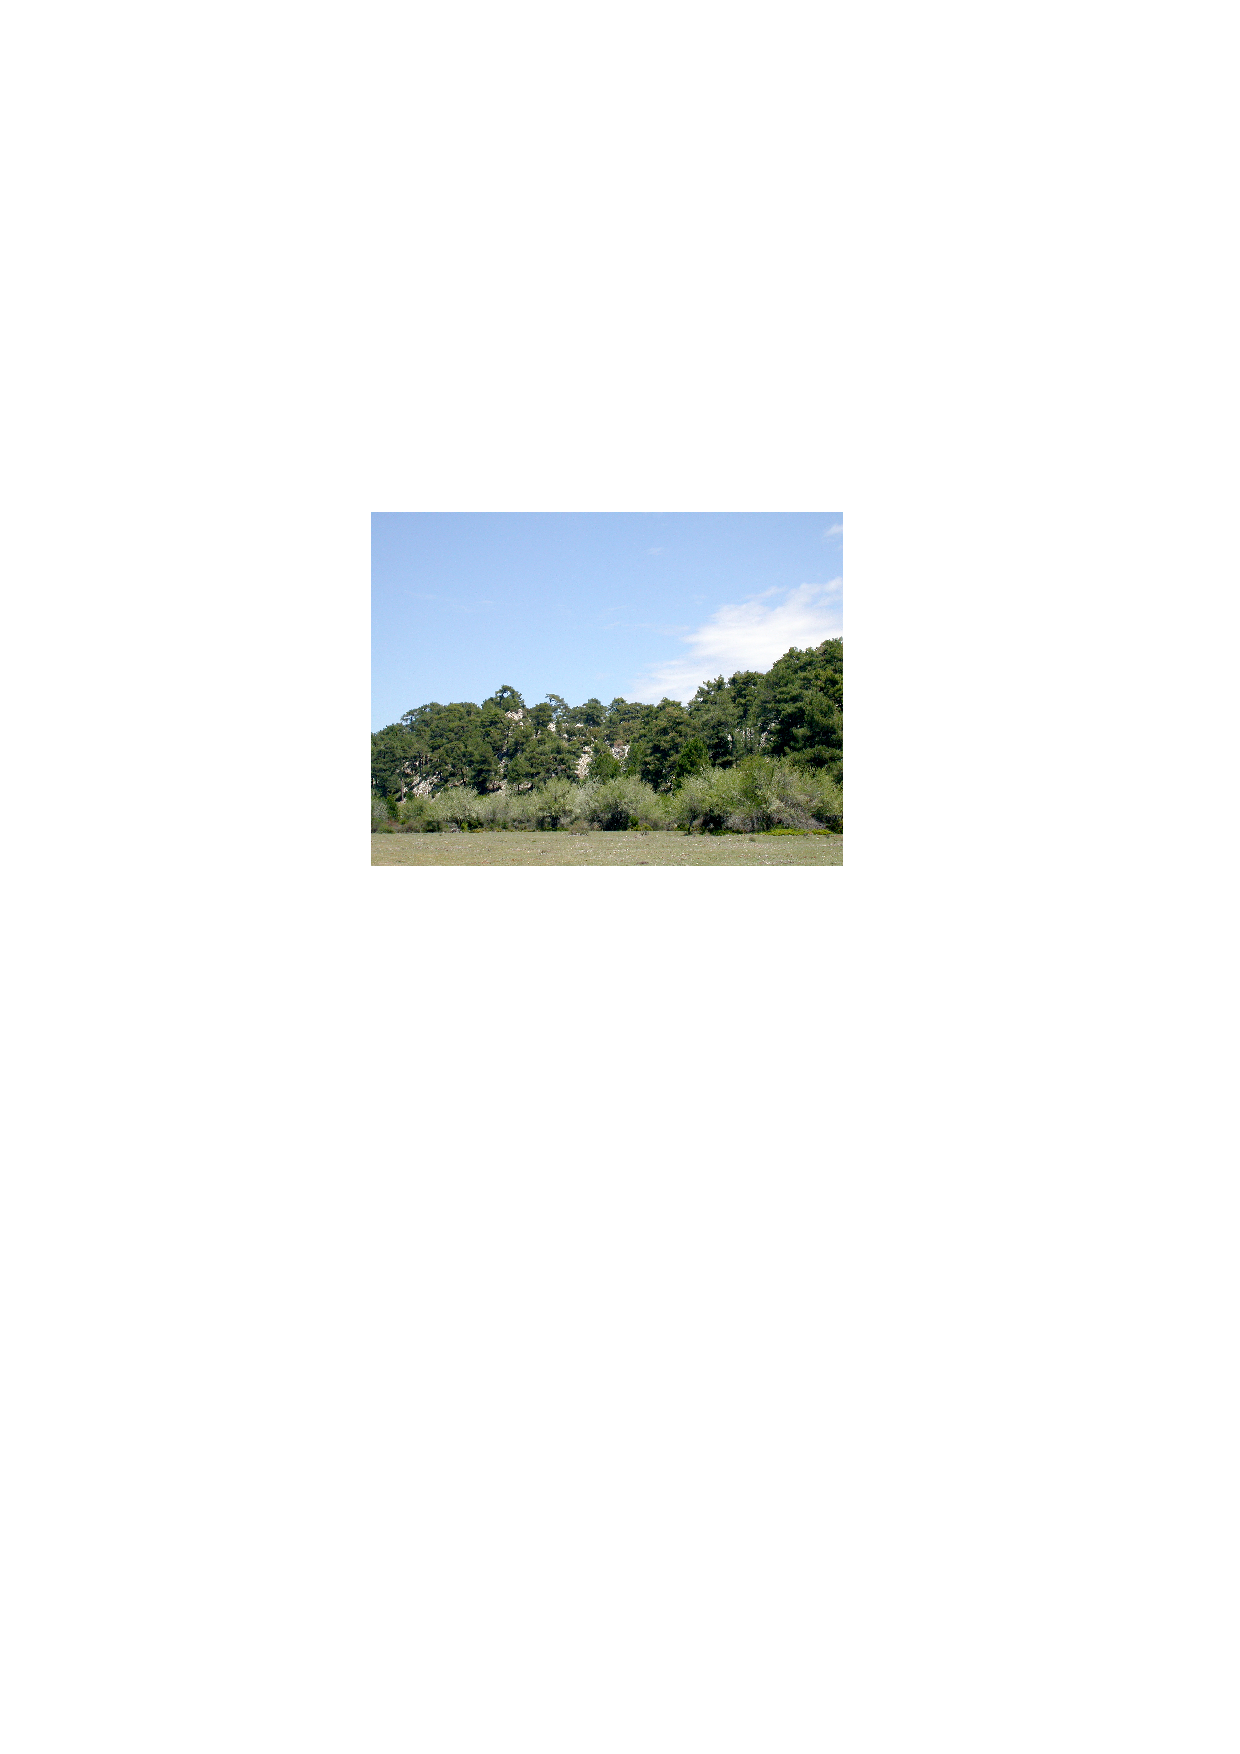
\includegraphics[height=10cm]{fig2.pdf}}
%
\caption{General view of the study area; late May, 2005. \textit{P. 
mahaleb} trees are flowering, with small white flowers, growing 
in the deep soil of the `nava', surrounded by rocky slopes with 
open pine-juniper forest.}
\end{figure}
%------------------------------------------------------------------- Figure 2

\tab Frugivorous birds and mammals visiting \textit{P. mahaleb} trees in Spanish populations usually behave as legitimate seed dispersers swallowing the fruits whole and defecating and/or regurgitating the seeds, usually after leaving the tree. Most seed rain of \textit{P. mahaleb} in the study areas is contributed by frugivorous birds. Seed rain and the resulting recruitment pattern of seedlings and saplings are highly patchy, and largely restricted to microhabitats beneath woody cover in the vicinity of fruiting trees (Jordano \& Schupp 2000).


\section{General approach to the direct estimation of seed dispersal 
distances}

\tab Our general approach is to compare the multilocus gentoype of the endocarp of dispersed seeds (either defecated or regurgitated by frugivorous animals) with those of potential maternal source trees in the population. Both hermaphrodite and female trees can act as seed sources in the study population, while only hermaphrodites act as pollen donors. The sex ratio is \ensuremath{\sim}1:1 for the two gender types in this population. The endocarp is a maternal tissue (2n) with an identical genotype to the mother tree (Fig. 3). In \textit{Prunus} it is derived from the carpellar wall. Thus, a full matching of the multilocus genotypes of a dispersed seed and a maternal tree unequivocally identifies the tree as the source for the dispersed seed, enabling a direct estimation of the dispersal distance (Fig. 4).


%------------------------------------------------------------------- Figure 3
\begin{figure}[htbp]
\centerline{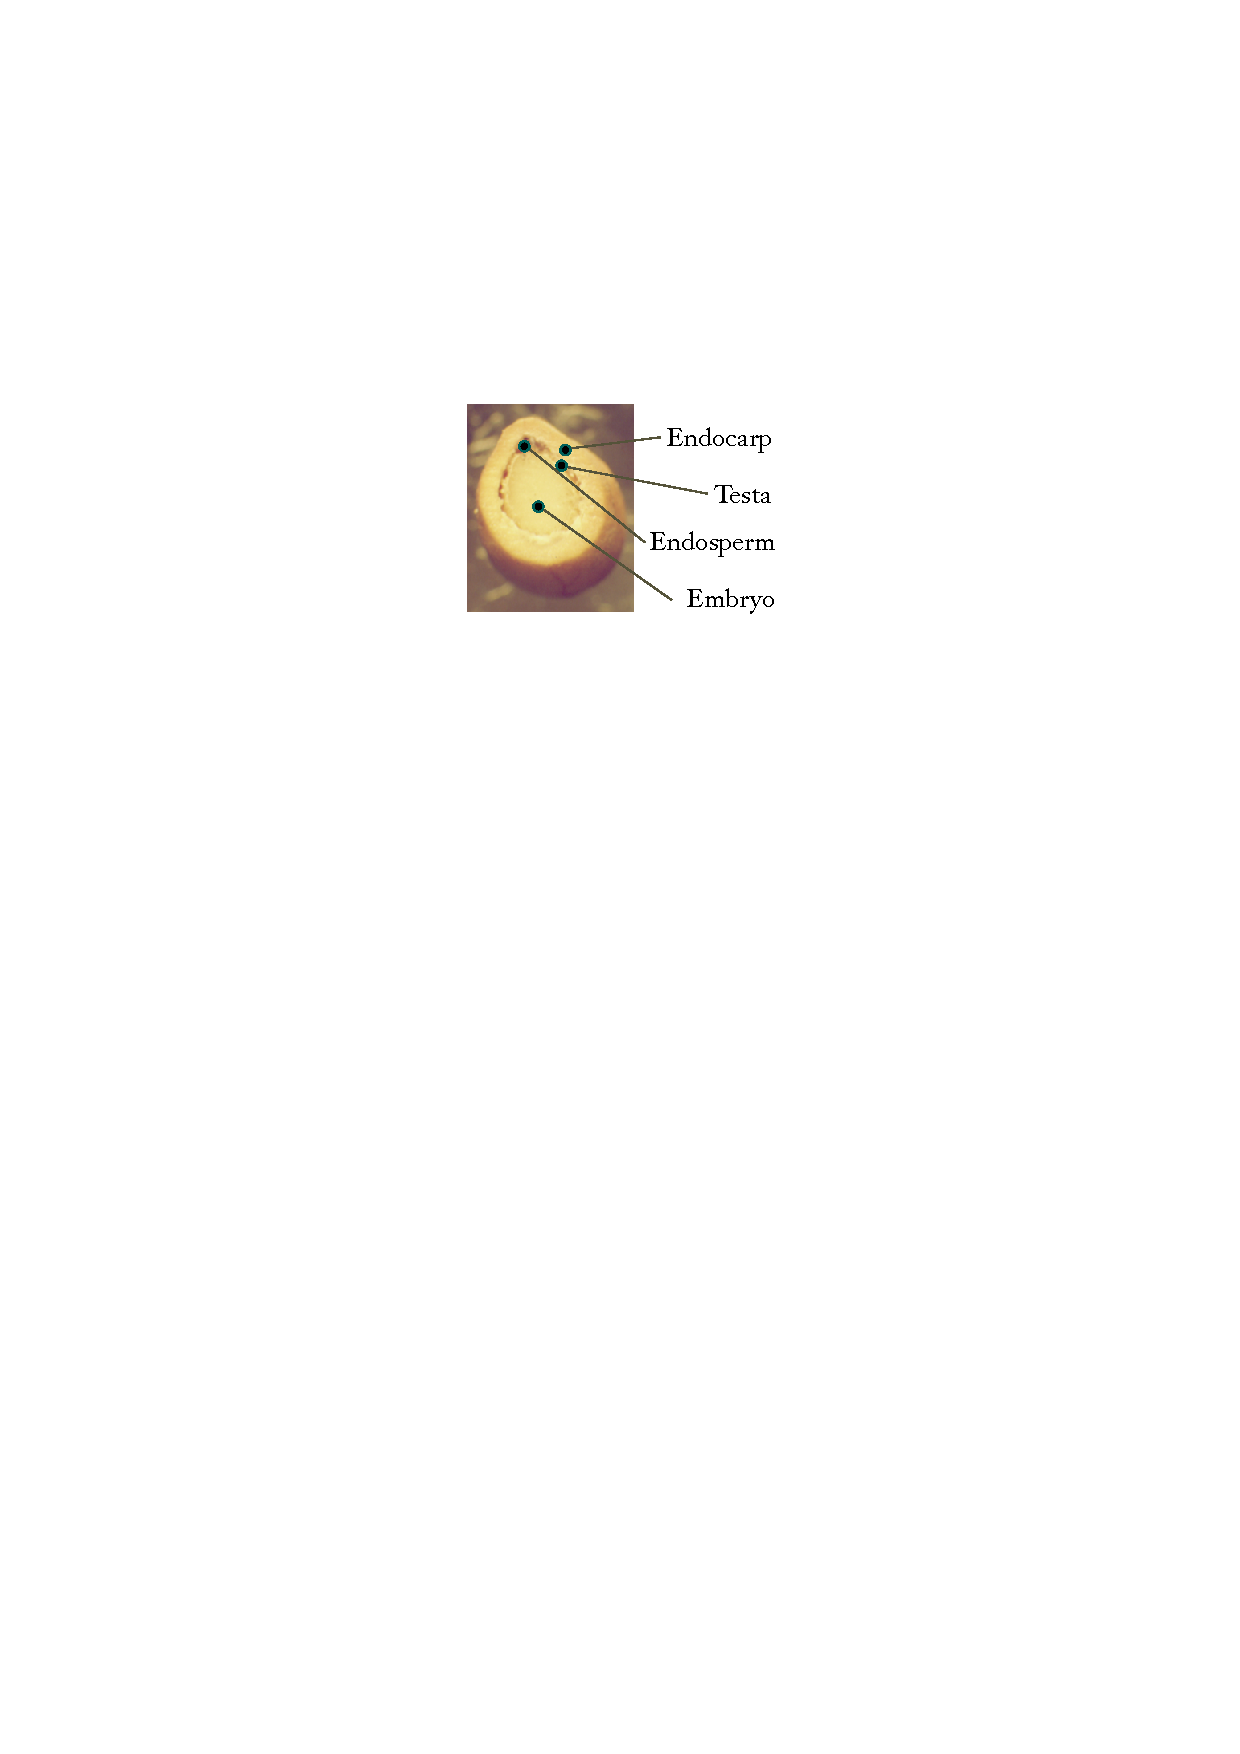
\includegraphics[height=4cm]{fig3.pdf}}
%
\caption{Cross section view of a \textit{P. mahaleb}} {\small seed showing the endocarp wall, consisting of wooody tissue and a central embryo filling up the whole seed interior. The seed is \ensuremath{\sim}5.5 mm maximum cross section, and the endocarp thickness is \ensuremath{\sim}1.5 mm.}
\end{figure}
%------------------------------------------------------------------- Figure 3

\tab {\small We have been separately genotyping also the testa tissue; in \textit{Prunus}} {\small this is a thin tissue just beneath the endocarp and overlying the embryo. In our analyses we carefully separated the testa when extracting the embryo to get only the endocarp material before homogeneization. The DNA yield of the testa was inssuficient to unequivocally determine its genotype, but we suspect it is also maternally-derived tissue. The embryo is, of course, a distinct diploid (2n) tissue with a contribution of the pollen-donor and a maternal contribution. Then the endosperm is triploid (3n) tissue with a single paternal contribution and two maternal contributions; in a ripe, fully-developed \textit{Prunus}} {\small seed it is vestigial. As the seed grows, the embryo displaces the endosperm towards the apical pole so that only a small amount remains in a fully developed, viable seed. \\ \tab To test the identity of the maternal genotype obtained from leaf tissue and the genotype of the seed endocarp, we sampled 1-3 seeds from the branches of 4 trees. In addition, we obtained the endocarp and embryo tissues from 11 seeds among the progeny (5 families) obtained in a diallel cross of known sires and dams obtained in 1992 and 1993; independent DNA extractions and genotypes were obtained from each tissue (P. Jordano, pers. obs.). Thus, for these seeds both the sire and dam trees were known and this allowed us to check the exact matching of the endocarp and leaf genotypes. When comparing embryo to parental genotypes, a strict Mendelian inheritance was observed with no evidence for the occurrence of null alleles (Godoy \& Jordano 2001).}

%------------------------------------------------------------------- Figure 4
\begin{figure}[htbp]
\centerline{\includegraphics[height=10cm]{fig4.pdf}}
%
\caption{View of the study area with adult \textit{P. mahaleb}} {\small fruiting trees and schematic, idealized, locations of pairs of seed traps (gray squares) in different microhabitats. Yellow arrows indicate assignments of seeds sampled in traps to their maternal trees, allowing an estimate of dispersal distance (\textit{d}) for each one. A fraction of the seeds sampled do not match any of the adult trees in the population (marked with ?) and are attributed to long-distance dispersal events, i.e., immigrant seeds originating in other populations.}
\end{figure}%------------------------------------------------------------------- Figure 4

\tab We genotyped 472 trees in the 9 populations, including all the 196 adult trees from the main study site, NCH, increasing our previous sample for this population (Godoy \& Jordano 2001). In this previous study we sampled leaf tissue for total of 180 adult trees, representing all the reproductives in the main nucleus of the population, during the years 1996-2000. We then added 16 trees in a patch ca. 300 m to the NW, thus totalling all the repoductives in the population. Our population consists of 104 hermaphrodite and 92 female trees scattered and patchily distributed (Fig. 5). We have also genotyped 84 additional young trees that were not reproducing in the 2003 season, totalling 263 individuals in NCH.

\tab Seeds dispersed by animals were sampled by setting replicates of 2 seed traps each at different randomly-chosen locations in NCH population (Fig. 5), stratified according to microhabitat type: beneath \textit{P. mahaleb} trees or other high shrubs (up to 4 m), beneath low shrubs (\texttt{} 1m height), beneath pine trees either with or without juniper understory, beneath trees with non-endozoochorous dispersed seeds (\textit{Acer}, \textit{Quercus}), in open ground with grassy cover, and in rocky substrates (see Jordano \& Schupp 2000). The adult reproductive trees in the population were mapped and their locations recorded in a GIS database including also the locations of the sampling sites with seed traps (Fig. 5).

 
%------------------------------------------------------------------- Figure 5
\begin{figure}[htbp]
\centerline{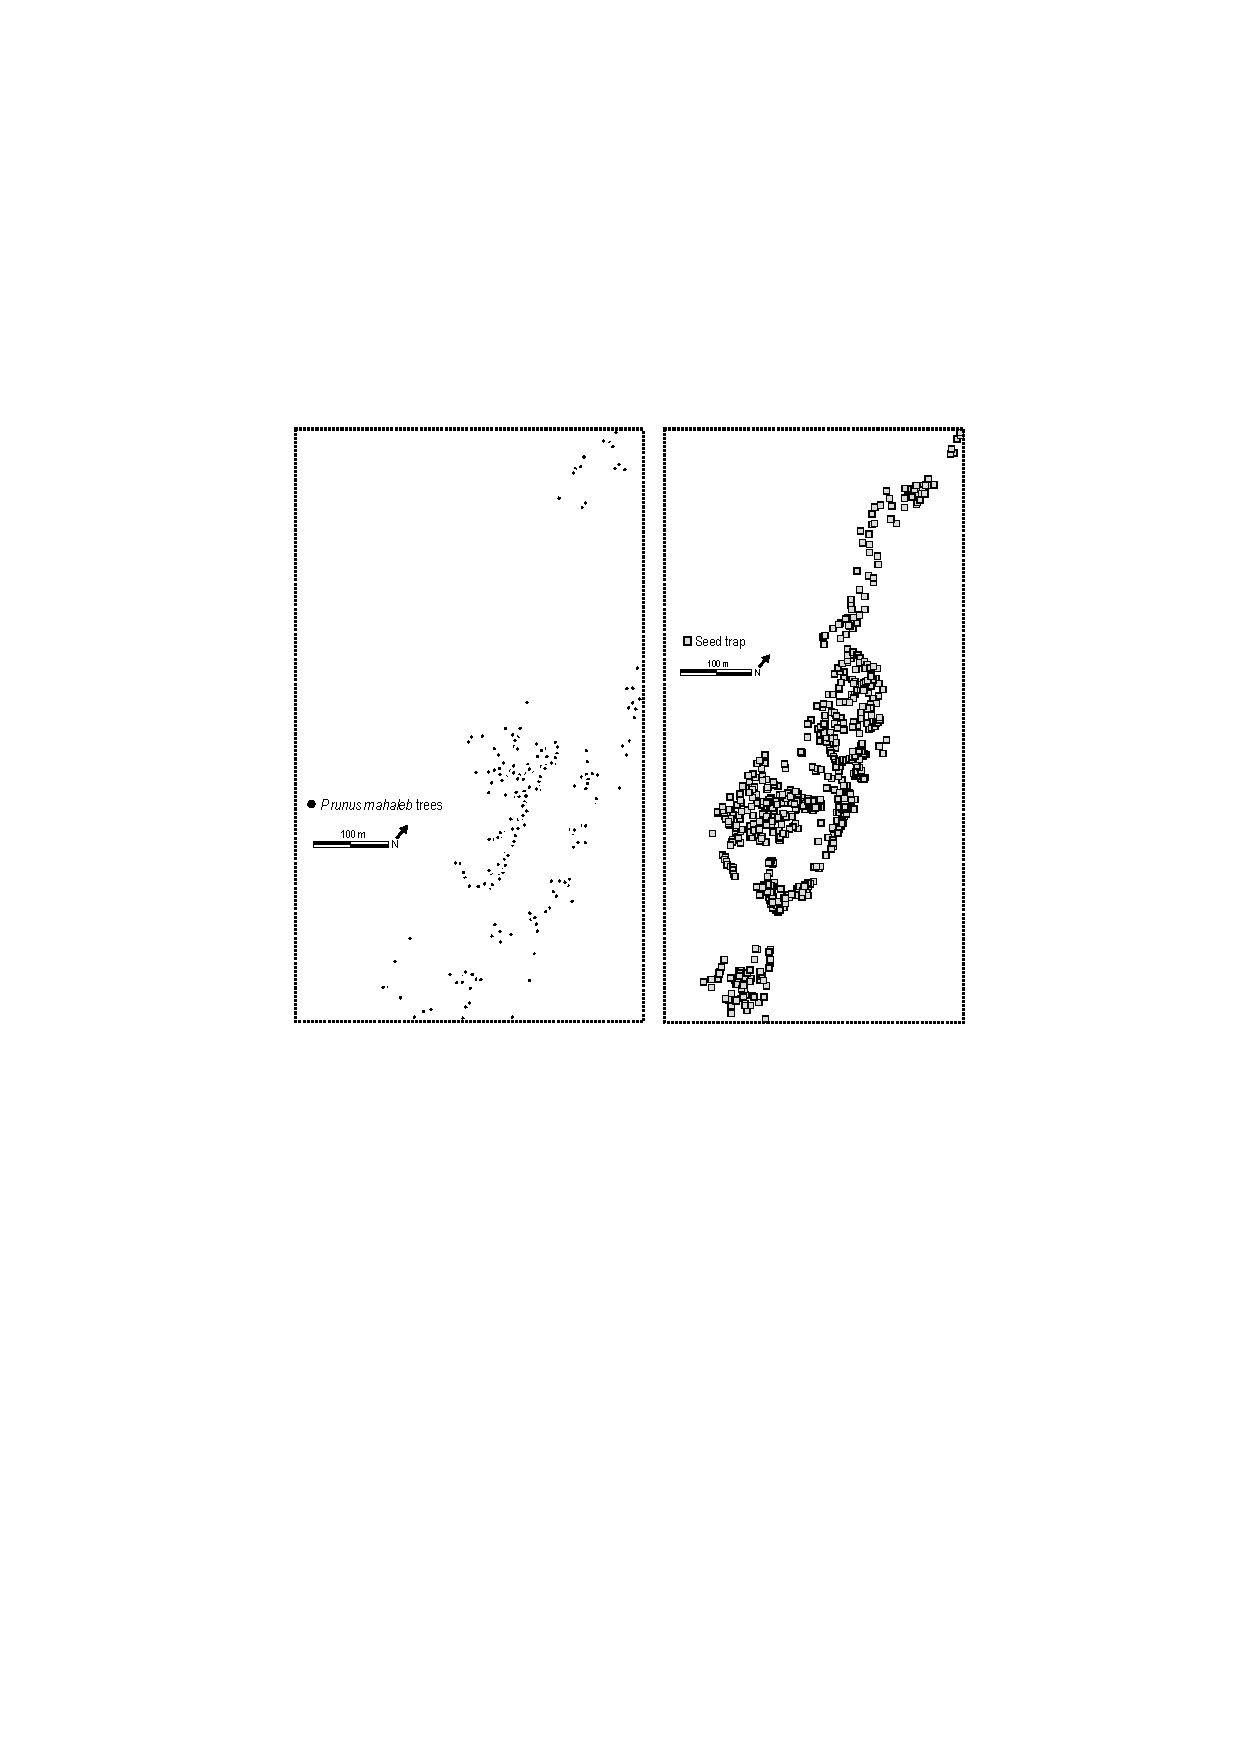
\includegraphics[height=10cm]{fig5.pdf}}
%
\caption{Map of the study area with adult \textit{P. mahaleb}} {\small fruiting trees (\textit{N}}{\small = 196) (left) and the locations of pairs of seed traps (\textit{N}}{\small = 613) (gray squares, right) in different microhabitats.}
\end{figure}%------------------------------------------------------------------- Figure 5

\tab Leaves (small pieces ca. 6 mm diameter) were frozen in liquid nitrogen after sampling and kept at -80 \ensuremath{^\circ}C until analysis. Seeds were air dried fater sampling and then dessicated in a forced-air oven at \texttt{}25 \ensuremath{^\circ}C. They were stored in paper bags until extraction of the endocarps. Dessication at higher temperatures damages the seeds and results in a reduced DNA extraction and amplification success.


\section{DNA extraction and microsatellite genotyping}

\tab DNA was extracted from 100-200 mg of fresh leaf tissue, sampled in 1998-1999, using the rapid miniprep method of Cheung \textit{et al}. (1993). We had additional sampling of leaves in 2000. We collected leaf pieces directly from the trees in individual Eppendorf tubes and immediately preserved them frozen in liquid nitrogen. Tissue was homogenized in 320 \ensuremath{\mu}L of extraction buffer (200 mM Tris-HCl pH 8.0, 70 mM EDTA, 2 M NaCl, 20 mM sodium bisulfite) with an electric drill (560 W; full speed) with attached plastic disposable pestles (see below for a modification of this grinding protocol). After homogenization 80 \ensuremath{\mu}L of 5\% sarcosyl was added and the sample was incubated at 65 \ensuremath{^\circ}C for 30 min and centrifuged at 16000 g for 15 min to remove insoluble material. DNA was precipitated by the addition of 90 \ensuremath{\mu}l of 10 M ammonium acetate and 200 \ensuremath{\mu}l of isopropanol. The mixture was incubated at room temperature for 5 min and centrifuged for 15 min at 16000 g. The pellet was washed with 70\% ethanol, dried and resuspended in 100 \ensuremath{\mu}L TE buffer. For the seed endocarps we used a similar protocol with some modifications. An important modification that we introduced since 2001 was the homogeneization of the endocarp tissue with a Rensch electronic grinder (Fig. 6). This increased the DNA yield and we now routinely use this grinder for all types of tissue. The endocarp tissue was introduced in an Eppendorf tube with 1 steel bead, frozen in liquid-nitrogen and grinded for at least 3 min at maximum speed. Tissue was homogenized in 480 \ensuremath{\mu}L of extraction buffer, 120 \ensuremath{\mu}L of 5\% sarcosyl was added, the sample was precipitated in 225 \ensuremath{\mu}L of 10 M ammonium acetate, and the DNA finally resuspended in 200 \ensuremath{\mu}L TLE (200 mM Tris-HCl pH 8.0, 70 mM EDTA).

%------------------------------------------------------------------- Figure 6
\begin{figure}[htbp]
\centerline{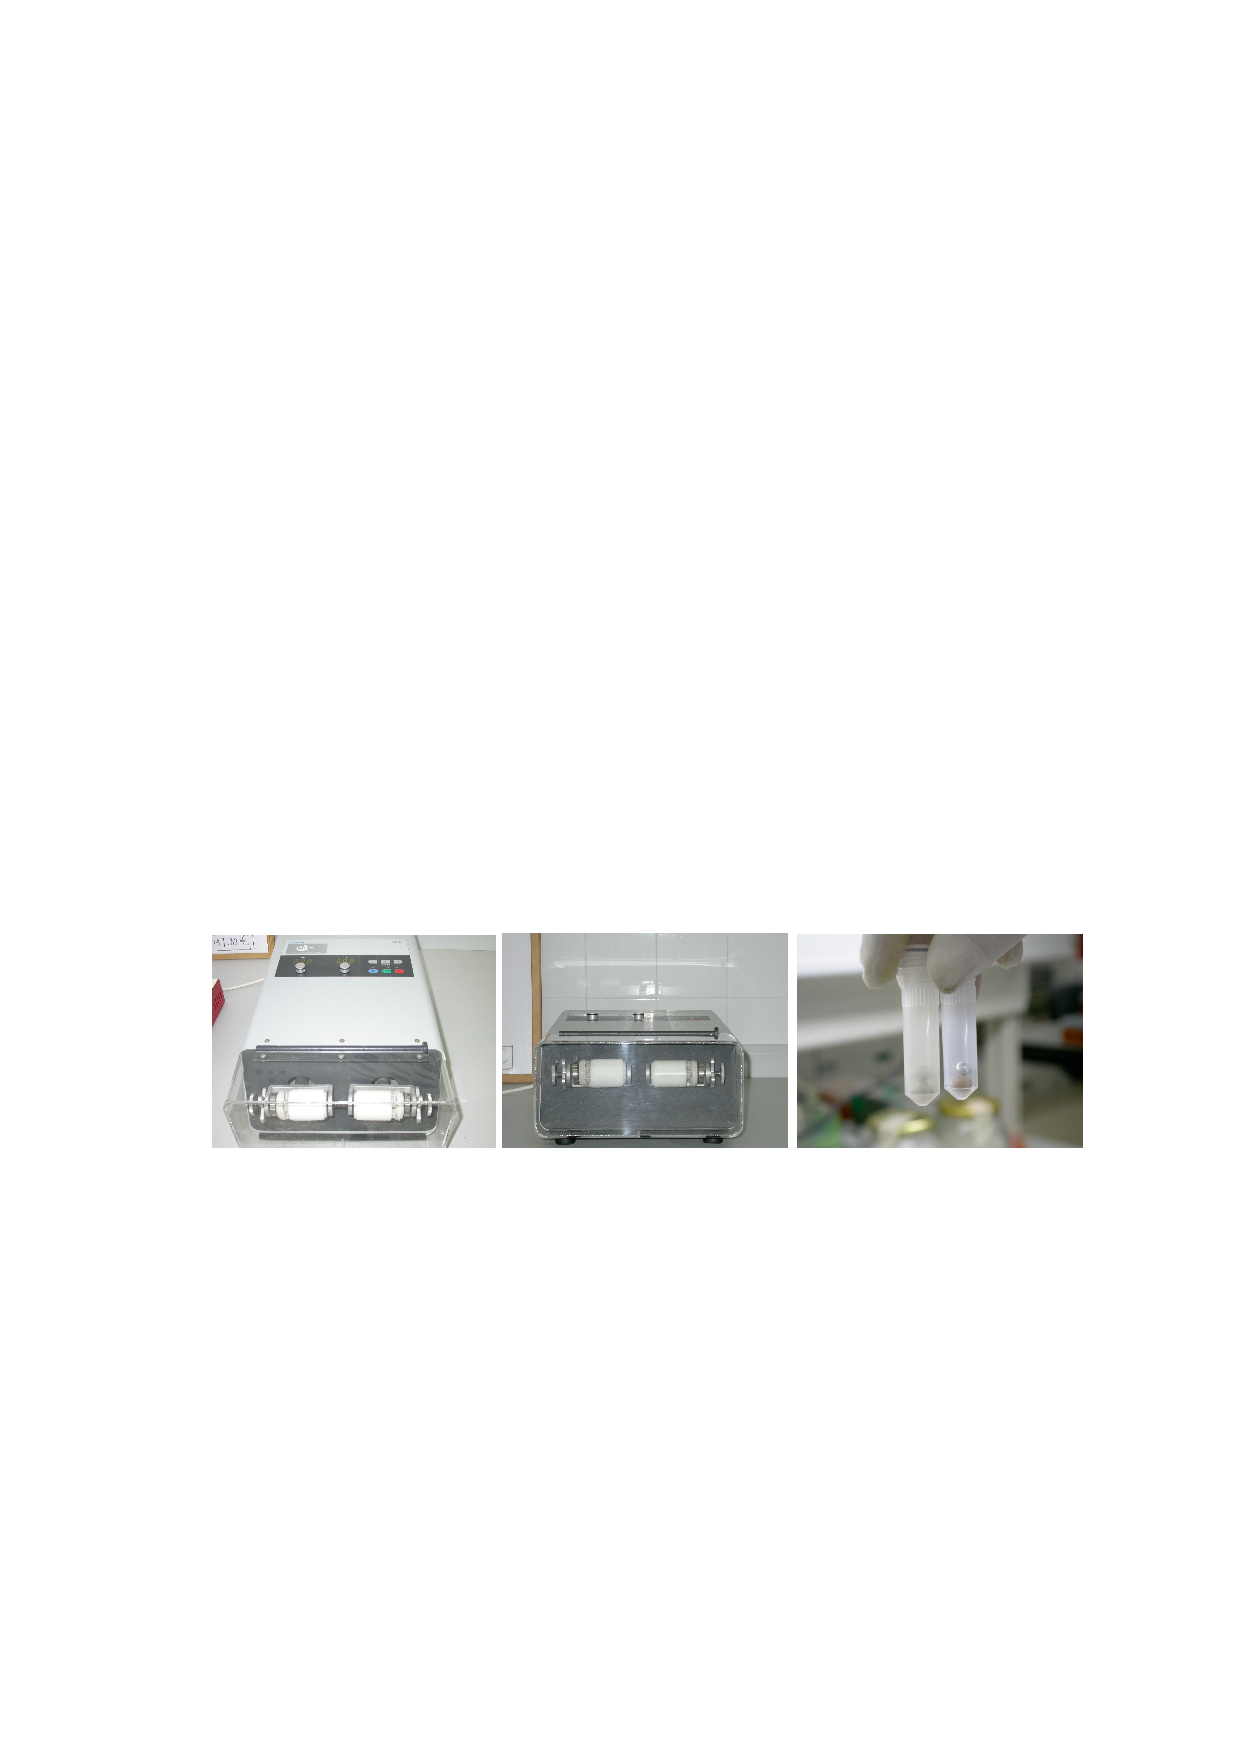
\includegraphics[height=3.5cm]{fig6.pdf}}
%
\caption{Two views of the electronic grinder (left) and two Eppendorff tubes with a seed and metallic ball (right) and the homogeneized endocarp fater grinding (left).}
\end{figure}%------------------------------------------------------------------- Figure 6

\tab We tested a total of 43 primers pairs designed for cultivated \textit{Prunus} and \textit{Malus} species (A. Abbott, 1998, personal communication; G. King, 1998, personal communication; Cipriani et al. 1999; Downey \& Iezzoni 2000; Sosinski et al. 2000). Of them 16 showed polymorphism when tested on 8 \textit{P. mahaleb} individuals of several populations. We finally selected a subset of 11 markers that showed polymorphism in \textit{P. mahaleb} for use in our project (Table 1).

%-------------------------------------------------------------------- Table 1

\begin{table}
\captionsetup{width=14cm}
\caption{Published names and references for the SSR microsatellite markers used in the study of \textit{Prunus mahaleb.}}

\vspace{0.5cm}
\begin{tabular}{cl}
\hline 
UDP96-001 & Aranzana, M. J., A. Pineda, P. Cosson, E. Dirlewanger, J. Ascasibar, G. Cipriani, C. D. Ryder, R. Testolin, A. Abbott, G. J. King, A. F. Iezzoni, and P. Arus. 2003. A set of simple-sequence repeat (SSR) markers covering the \textit{Prunus} genome. Theoretical and Applied Genetics \textbf{106}: 819-825. \\UDP96-018 &  \\UDP97-403 &  \\UDP97-406 &  \\UDP97-402 & Cipriani, G., G. Lot, W. G. Huang, M. T. Marrazzo, E. Peterlunger, and R. Testolin. 1999. AC/GT and AG/CT microsatellite repeats in peach [\textit{Prunus persica} (L) Batsch]: isolation, characterisation and cross-species amplification in Prunus. Theoretical and Applied Genetics \textbf{99}: 65-72. \\pchgms3 & Sosinski, B., M. Gannavarapu, L. D. Hager, L. E. Beck, G. J. King, C. D. Ryder, S. Rajapakse, W. V. Baird, R. E. Ballard, and A. G. Abbott. 2000. Characterization of microsatellite markers in peach [\textit{Prunus persica} (L.) Batsch]. Theoretical and Applied Genetics \textbf{101}: 421-428. \\PS12A02 &  \\pchcms 5 & Downey, S. L., and A. F. Iezzoni. 2000. Polymorphic DNA markers in black cherry (\textit{Prunus serotina}) are identified using sequences from sweet cherry, peach, and sour cherry. Journal of the American Society of Horticultural ScienceJ. \textbf{125}: 76-80. \\pchcms4 &  \\PS01H03 &  \\
\hline
%\toprule
\end{tabular}
\end{table}
%-------------------------------------------------------------------- Table 1

\tab We used the full set of 11 markers for the adult trees, but only used 9 markers for the endocarps due to limited success with amplifications from endocarp tissue for some of the markers. Thus, markers were selected not only because of their polymorphism levels but also to optimize the muiltiplexing in the sequencer, that is, the possibility of running groups of markers, with non-overlapping size ranges, at a time in the sequencer. We designed 3 groups of markers with non-overlapping allelic sizes. Each group was labelled with a distinct fluorescent marker (5' Fam, 5' Tet or 5' Hex) and each locus is amplified in an independent PCR reaction. The amplified products are mixed in adequate proportions and analyzed in the Applied Biosystems Model 310. With the set of microsatellite markers used, each adult tree in the population showed a unique multilocus genotype.

\tab Polymerase chain reaction (PCR) amplification was performed in 20 \ensuremath{\mu}l reaction volumes containing 67 \ensuremath{\mu}M Tris-HCl pH 8.8, 16 mM $(NH_{4})2SO_{4}$, 2 \ensuremath{\mu}M $MgCl_2$, 0.01\% Tween-20, 0.01\% BSA, 0.25 mM of each dNTP, 0.25 \ensuremath{\mu}M of each primer, 0.5 U of Taq DNA polimerase, and 10.8 \ensuremath{\mu}l H2O. Reactions were incubated in a MJ Research PTC-100 thermocycler programmed for a ``touchdown'' PCR as follows: an initial denaturation step at 94\ensuremath{^\circ} C for 2 min; 16 cycles of 92\ensuremath{^\circ} C for 30 s, annealing at 66-50\ensuremath{^\circ} C for 30 s (1\ensuremath{^\circ} C decrease in each cycle), and extension at 72\ensuremath{^\circ} C for 30 s; 19 cycles of 92\ensuremath{^\circ} C for 30 s, 50\ensuremath{^\circ} C for 30 s, and 72\ensuremath{^\circ} C for 30 s (Table 2). A final extension was programmed at 72\ensuremath{^\circ} C for 5 min. Amplified fragments were analyzed using a capillary electrophoresis automated sequencer, ABI 3100 Genetic Analyser (Applied Biosystems). We are currently using this Applied Biosystems Model 3100 sequencer and we label with 5'Fam, 5'Net and 5'Hex fluorescent markers. Previously we used an ABI 377 model. We scored the electropherograms using Genescan 3.1 and Genotyper 3.7 (Applied Biosystems). The scorings were checked haphazardly and separately by two people for consistency. In several cases of doubtful assignements we re-run all the genotyping protocol for the sample.

%--------------------------------------------------------------------- Table 2
\newpage
\pagestyle{empty}
\begin{landscape}
	%%%%%%%%%%%%%%%%%%%%%%%%%%%%%%
%	\oddsidemargin  0.0in
%	\evensidemargin 0.0in
%	\textwidth      8.5in
	\headheight     4.5cm
%	\topmargin      0.0in
%	\textheight=8.0in
	%%%%%%%%%%%%%%%%%%%%%%%%%%%%%%
\begin{table}
\captionsetup{width=21cm}%.75\textwidth}
\caption{Allele frequencies (N) for the 11 SSR microsatellite markers used. Alleles for each locus are identified by their size (bp).}

\vspace{0.5cm}
\begin{tabular}{rrrrrrrrrrrrrrrrrrrrrr}
\toprule

\multicolumn{ 2}{c}{Fam001} &     \multicolumn{ 2}{c}{FamMg3} &     \multicolumn{ 2}{c}{Fam018} &     \multicolumn{ 2}{c}{Tet403} &     \multicolumn{ 2}{c}{TetE02} &     \multicolumn{ 2}{c}{TetMC4} &     \multicolumn{ 2}{c}{TetMC5} &     \multicolumn{ 2}{c}{Hex406} &     \multicolumn{ 2}{c}{Hex402} &     \multicolumn{ 2}{c}{HexA05} &   \multicolumn{ 2}{c}{HexH03}\\ &            &            &            &            &            &            &            &            &            &            &            \\

    Allele &          N &     Allele &          N &     Allele &          N &     Allele &          N &     Allele &          N &     Allele &          N &     Allele &          N &     Allele &          N &     Allele &          N &     Allele &          N &     Allele &          N \\
\toprule

           &            &            &            &            &            &            &            &            &            &            &            &            &            &            &            &            &            &            &            &            &            \\

       109 &          9 &        176 &         24 &        244 &        204 &        102 &         30 &        143 &          1 &        221 &        237 &        231 &        296 &         93 &        110 &        116 &          2 &        194 &         53 &        249 &          4 \\

       117 &         64 &        178 &        195 &        246 &        216 &        104 &        225 &        145 &         14 &        222 &        109 &        235 &         96 &         95 &        136 &        118 &          5 &        196 &          1 &        251 &         18 \\

       119 &        292 &        186 &         25 &            &            &        106 &         22 &        153 &          1 &        226 &         31 &            &            &         97 &        167 &        132 &         88 &        198 &        273 &        255 &          1 \\

       121 &         30 &        190 &         28 &            &            &        110 &         16 &        159 &          1 &        228 &         41 &            &            &        101 &          5 &        134 &         29 &        200 &         86 &        257 &         72 \\

       125 &          2 &        192 &         19 &            &            &        112 &         23 &        161 &          8 &            &            &            &            &        107 &          2 &        136 &         65 &        202 &          7 &        259 &          9 \\

       127 &         20 &        194 &         73 &            &            &        116 &          8 &        167 &         79 &            &            &            &            &            &            &        138 &          1 &            &            &        261 &         41 \\

       129 &          3 &        196 &          6 &            &            &        118 &          2 &        169 &          8 &            &            &            &            &            &            &        142 &        140 &            &            &        263 &         19 \\

           &            &        200 &          1 &            &            &        122 &         26 &        173 &         90 &            &            &            &            &            &            &        144 &          6 &            &            &        267 &          1 \\

           &            &        204 &         18 &            &            &        124 &         31 &        175 &          2 &            &            &            &            &            &            &        146 &         79 &            &            &        269 &          3 \\

           &            &        206 &         31 &            &            &        142 &         37 &        177 &          3 &            &            &            &            &            &            &        148 &          5 &            &            &        271 &         55 \\

           &            &            &            &            &            &            &            &        183 &        188 &            &            &            &            &            &            &            &            &            &            &        273 &         11 \\

           &            &            &            &            &            &            &            &        185 &         11 &            &            &            &            &            &            &            &            &            &            &        275 &          2 \\

           &            &            &            &            &            &            &            &        187 &         14 &            &            &            &            &            &            &            &            &            &            &        281 &          1 \\

           &            &            &            &            &            &            &            &            &            &            &            &            &            &            &            &            &            &            &            &        283 &        100 \\

           &            &            &            &            &            &            &            &            &            &            &            &            &            &            &            &            &            &            &            &        287 &         19 \\

           &            &            &            &            &            &            &            &            &            &            &            &            &            &            &            &            &            &            &            &        289 &         20 \\

           &            &            &            &            &            &            &            &            &            &            &            &            &            &            &            &            &            &            &            &        291 &          1 \\

           &            &            &            &            &            &            &            &            &            &            &            &            &            &            &            &            &            &            &            &        295 &         42 \\

           &            &            &            &            &            &            &            &            &            &            &            &            &            &            &            &            &            &            &            &        297 &          1 \\
\toprule
\end{tabular}
\end{table}
\end{landscape}
%--------------------------------------------------------------------- Table 2

%--------------------------------------------------------------------- Table 3
\begin{table}
%\captionsetup{width=20cm}%.75\textwidth}
\caption{Summary of the PCR program protocol.}
\vspace{0.2cm}

\begin{tabular}{lcl}

\toprule
Step  &  Temperature  &       Time \\
\toprule
1- initial denaturalization  &  94 \ensuremath{^\circ} C  &      2 min \\
2- denaturalization  &  92 \ensuremath{^\circ} C  &       30 s \\
3- annealing  &  66 \ensuremath{^\circ} C -- 1\ensuremath{^\circ}C / cycle  &       30 s \\
4- extension  &  72 \ensuremath{^\circ} C  &       30 s \\
5- repeated cycles  &  17 cycles of steps 2 to 4  &            \\
6- denaturalization  &  92 \ensuremath{^\circ} C  &       30 s \\
7- annealing  &  50 \ensuremath{^\circ} C  &       30 s \\
8- extension  &  72 \ensuremath{^\circ} C  &       30 s \\
9- repeated cycles  &  18 cycles of steps 6 to 8  &            \\
10- final extension  &  72 \ensuremath{^\circ} C  &      5 min \\
11- refrigeration  &  4 \ensuremath{^\circ} C  &  indefinite \\
\toprule
\end{tabular}
\end{table}
%--------------------------------------------------------------------- Table 3

\section{Source tree identification}

\tab For the study of seed dispersal, a total of 180 adult trees and 95 dispersed seed endocarps were initially genotyped (Godoy \& Jordano 2001). We have later expanded this sample to include 263 trees from NCH (of which we use only the 196 reproductives in 2003) and 557 endocarps and this is currently (March 15, 2005) our main analysis dataset. We have also genotyped trees from other 8 populations in addition to NCH, totalling 472 trees. A total of 21 endocarps failed to amplify for \ensuremath{\geq} 3 loci and were dropped from analyses.

\tab Each adult tree in the NCH population showed a unique multilocus genotype. The source tree for individual dispersed seeds was identified by comparing the endocarp multilocus genotype with the complete set of genotypes of reproductive trees in the population. To assign the source tree for each dispersed seed we carried out an identity check by matching the multilocus genotype of the endocarp at 9 microsatellite loci with those of the adult trees; for the adult trees we assessed 11 SSR loci. We used the full seed sample from the 1996 (\textit{N}= 95) and 1997 (\textit{N}= 462) seed cohorts. We used CERVUS (Marshall \textit{et al}. 1998) and GIMLET (Vali\`{e}re 2002) to identify the mismatches and multiple-matches among endocarps and putative source trees.

\tab For each sampled seed, the adult individual having a genotype matching the seed endocarp genotype was assigned as the mother tree. In a few cases (\textit{N}= 27 endocarps) we failed to find evidence that a NCH tree was mother source, yet they had \ensuremath{\leq} 2 loci missing and thus we were unable to assign them as immigrant seeds in NCH and we consider them re-assigned NCH seeds. All the seed endocarps except 2 (among those matching NCH tree genotypes) were assigned to a single tree in NCH; 97 endocarps were not assignable to any tree in NCH. Finally, 27 endocarps were dropped from analysis due to amplification failure for \texttt{}2 loci. We thus had 474 endocarps assigned to the NCH study population. The two seeds with double matching have failed amplifications for two loci and resulted in ambiguous matchig with two putative maternal trees. We assigned the seeds to the tree nearest to the sampling location, due to the fact that this procedure would minimize the estimation errors of dispersal distances when these are distributed with high skew, i.e., a missassignment of a rare long-distance event would seriously bias the estimate of the dispersal function. Significant matches between endocarp and adult genotypes were found by testing a hypothesis of identity ($r_{p}= 1$, $r_{m}= 1$) in all possible pairwise comparisons between endocarps and adult trees and obtaining significance estimates by a jackknife resampling method (Queller \& Goodnight 1989). 

\section{Problems with SSR genotyping}

\tab There can be some problems at the genotyping and assignment stages when working with seed endocarps, and some of them are quite frequent in paternity analyses. First, stutter bands. They are fairly common when analyzing microstellites, specially with dinucleotide repeats. We have them in amplifications from endocarp extracts but also, and to the same extent, with leaf extracts and with all other species we have worked with. Alleles were assigned to the largest, and most abundant, fragment. Heterozygotes for two close alleles were recognized by the shortest allele showing a higher intensity than the larger (the intensity of the band being the sum of the short allele and the stutter bands of the long allele). This results in a characteristic pattern clearly distinguishable from the homozygote pattern, in which the intensity of the bands decreases progressively with size. This is described in Hoelzel (1998). We think touchdown PCR will not alleviate the problem of stutter bands. We use it to prevent non-specific products in our heterologous amplifications.

\tab Second, null alleles and allelic dropout. Null alleles are alleles that do not amplify, probably because of a mismatch in one of the primers used. They can be suspected if a heterozygote deficit is detected only in some of the loci; they are frequent in paternity analysis (Bj\"{o}rklund 2005). If null alleles are present, they should appear \textit{both} in leaf and endocarp extracts. Therefore, we don't think they would affect the identity checks between seeds and trees, a seed showing a false homozygote will match a tree showing the same pattern. However, this will affect and limit the resolution power and bias the significance values for assignements (see below). We did not discard that null alleles were present in our samples, but we didn't find them. We observed an heterozigote deficit but in most loci, resulting from high inbreeding in the study population due to frequent selfing. We have not detected null alleles in a few paternity analyses where we used progeny with known paternal and maternal trees, obtained from hand pollinations.

\tab Finally, allelic dropout can be a serious problem for the assignment of seeds to mother trees. It occurs when one of the alleles in an heterozygote is not amplified stochastically when using limiting amounts of template DNA, as can be the case when endocarp extracts are used. In the controlled comparisons we made between leaf and endocarp genotypes, allelic dropout was not observed. But this can be a potential problem if the DNA yield or quality is limiting. Repeating the amplification of homozygote loci several times (Taberlet 1996) and accurately determining the concentration of DNA and excluding those samples in the limiting range where allelic dropout can occur (Morin \textit{et al. }2001) are two strategies to deal with the problem at the genotyping stage. At the analysis level, any exclusion of identity between a seed and a potential mother tree based on only 1 or 2 loci mismatching was rechecked.

%%%%%%%%%%%%%%%%%%%%%%%%%%%%%%%%%%%%%%%%%%%%%%%%%%%%%%%%%%%%%%%%% BIBLIOGRAPHY
\begin{thebibliography}{1}

\bibitem{item1}Bj\"{o}rklund M. 2005 A method for adjusting allele frequencies 
in the case of microsatellite allele drop-out. Molecular Ecology Notes \textbf{5}: 676-679.

\bibitem{item2}Cheung, W. Y., N. Hubert, and B. S. Landry. 1993. A simple and 
rapid DNA microextraction method for plant, animal, and insect suitable for RAPD and PCR analyses. PCR Methods and Applications 
\textbf{3}: 69-70.

\bibitem{item3}Godoy, J. A., and P. Jordano. 2001. Seed dispersal by animals: 
exact identification of source trees with endocarp DNA microsatellites. Molecular Ecology \textbf{10}: 2275-2283.

\bibitem{item4}Grivet, D., P.E. Smouse, and V.L. Sork. 2005. A novel approach 
to an old problem: tracking dispersed seeds. Molecular Ecology \textbf{14}: 3585-3595.

\bibitem{item5}Hoelzel, A.R. 1998. \textit{Molecular genetic analysis of populations: a practical approach}. Oxfrod University Press, Oxford, UK.

\bibitem{item6}Jones, A., J. Chen, G. J. Weng, and S. P. Hubbell. 2005. A genetic evaluation of seed dispersal in the Neotropical tree, \textit{Jacaranda 
copaia} (Bignoniaceae). American Naturalist \textbf{166}: 000-000. 
\textit{In press}.

\bibitem{item7}Jordano, P. 1994. Spatial and temporal variation in the avian-frugivore assemblage of \textit{Prunus mahaleb}: patterns and consequences. Oikos \textbf{71}: 479-491.

\bibitem{item8}Jordano, P. 1995. Frugivore-mediated selection on fruit and seed size: birds and St. Lucie's cherry, \textit{Prunus mahaleb}. Ecology 
\textbf{76}: 2627-2639.

\bibitem{item9}Jordano, P., and E. W. Schupp. 2000. Seed disperser effectiveness: the quantity component and patterns of seed rain for \textit{Prunus mahaleb}. Ecological Monographs \textbf{70}: 591-615.

\bibitem{item10}Jordano, P., and J. A. Godoy. 2002. Frugivore-generated seed 
shadows: a landscape view of demographic and genetic effects. Pages 305-321 \textit{in} D. J. Levey, W. Silva, and M. Galetti, editors. Frugivores and seed dispersal: ecological, evolutionary, and conservation issues. CAB International, Wallingford, UK.

\bibitem{item11}Marshall TC, Slate J, Kruuk LEB, Pemberton JM. 1998. Statistical confidence for likelihood-based paternity inference in natural 
populations. Molecular Ecology \textbf{7}: 639-655.

\bibitem{item12}Morin, P.A., K.E. Chambers, C. Boesch and L. Vigilant. 2001. 
Quantitative polymerase chain reaction analysis of DNA from non-invasive 
samples for accurate microsatellite genotyping of wild chimpanzees 
(\textit{Pan troglodytes verus}). Molecular Ecology \textbf{10}: 1835-1844.

\bibitem{item13}Taberlet, P. \textit{et al}. 1996. reliable genotyping of samples with very low DNA quantities using PCR. Nucleic Acids Research \textbf{24}: 3189-3194.

\bibitem{item14}Vali\`{e}re, N. 2002. GIMLET: a computer program for analysing 
genetic individual identification data. Molecular Ecology Notes \textbf{2}: 377--379.

\bibitem{item15}Ziegenhagen, B., S. Liepelt, V. Kuhlenkamp, and M. Fladung. 2003. Molecular identification of individual oak and fir trees from maternal tissues of their fruits or seeds. Trees-Structure and Function \textbf{17}: 345-350.

\end{thebibliography}

%\begin{flushright}
%{\footnotesize SSR genotyping protocols for \textit{Prunus mahaleb. }}{\footnotesize v. 1.1 - Jordano \& Godoy - 1.13}
%\end{flushright}

\end{document}
%%%%%%%%%%%%%%%%%%%%%%%%%%%%%%%%%%%%%%%%%%%%%%%%%%%%%%%%%%%%%%%%%%%%%%%%%%%%%%


